\documentclass[a4paper, 11pt]{article}%

%%%%%%%%%%%%%%%%%%%%%%%%%%%%%%%%%%%%%%%%%%%%%%%%%%%%%%%%%%%%%%%%%%%%%%%%

% Global structure parameters
\usepackage{fullpage}%

\usepackage[francais]{babel}%

\usepackage[utf8]{inputenc}%
\usepackage[T1]{fontenc}%

% Font selection
% (newpx n'a pas été installé avex TeXLive...)
\usepackage{mathpazo}%
\usepackage{courier}%

% Macro packages
\usepackage{url}%
\usepackage{graphicx}%
\usepackage{listings}%

\usepackage[font=scriptsize,labelfont=bf]{caption}

% Parameters for listings
\lstset{%
	basicstyle=\footnotesize\sffamily,%
	columns=fullflexible,%
	frame=lb,%
	frameround=fftf,%
	language=caml,%
}%

% Fine tuning
\setlength{\parskip}{0.5\baselineskip}%

%%%%%%%%%%%%%%%%%%%%%%%%%%%%%%%%%%%%%%%%%%%%%%%%%%%%%%%%%%%%%%%%%%%%%%%%

\begin{document}

\title{Rapport de projet}

\author{Marco Freire, Clément Legrand-Duchesne}

\date{26 septembre 2017}

\maketitle

\begin{abstract}
  Dans ce rapport seront expliqués les codes du pavage de Penrose et des
  tours de Hanoi, ainsi que leurs extensions; et les choix d'implémentation
  que nous avons été menés à faire.
\end{abstract}

%%%%%%%%%%%%%%%%%%%%%%%%%%%%%%%%%%%%%%%%%%%%%%%%%%%%%%%%%%%%%%%%%%%%%%%%

\section{Penrose}

\section{Hanoi}

	\subsection{Principe: algorithme de base}
		Le problème des tours de Hanoi est essentiellement récursif. Pour
		déplacer n disques du premier poteau jusqu'au troisième
		il suffit de savoir en déplacer n-1 sur le deuxième poteau (étape 1), puis
		de déplacer le n-ième disque sur le troisième poteau (étape 2) et enfin de
		déplacer encore une fois les n-1 disques sur le troisième poteau (étape 3).

		\begin{figure}[!h]
			\minipage{0.24\textwidth}
			  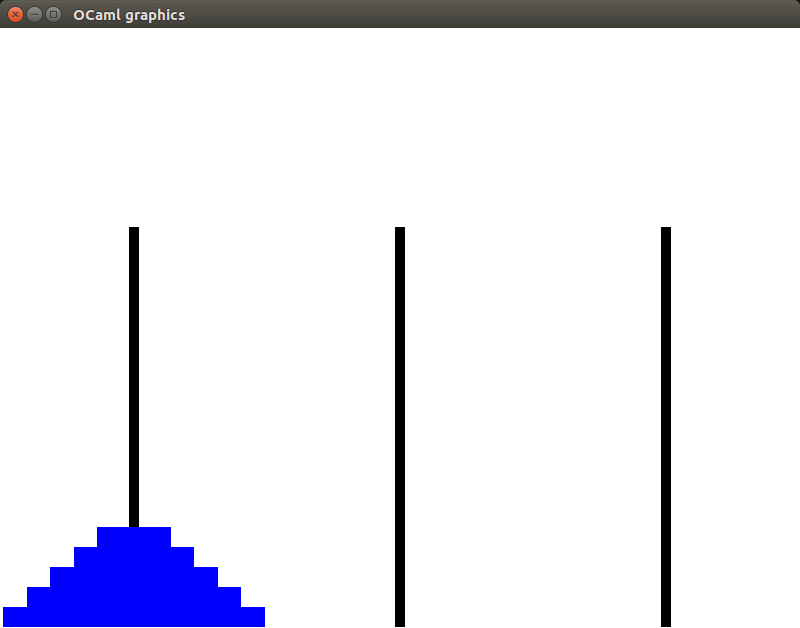
\includegraphics[width=\linewidth]{hanoi_start.png}
			  \caption{État initial}\label{fig:hanoi_start}
			\endminipage\hfill
			\minipage{0.24\textwidth}
			  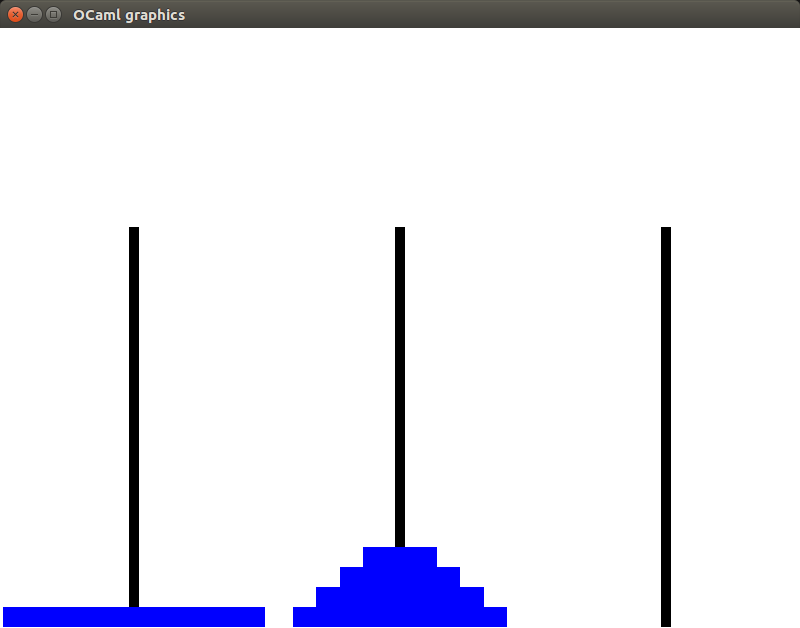
\includegraphics[width=\linewidth]{hanoi_mid1.png}
			  \caption{Fin étape 1}\label{fig:hanoi_mid1}
			\endminipage\hfill
			\minipage{0.24\textwidth}
			  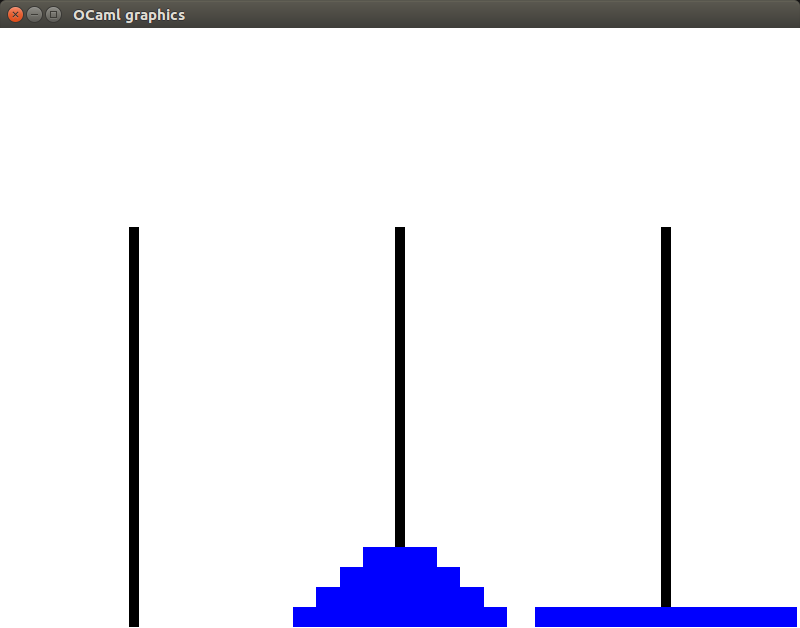
\includegraphics[width=\linewidth]{hanoi_mid2.png}
			  \caption{Fin étape 2}\label{fig:hanoi_mid2}
			\endminipage\hfill
			\minipage{0.24\textwidth}
			  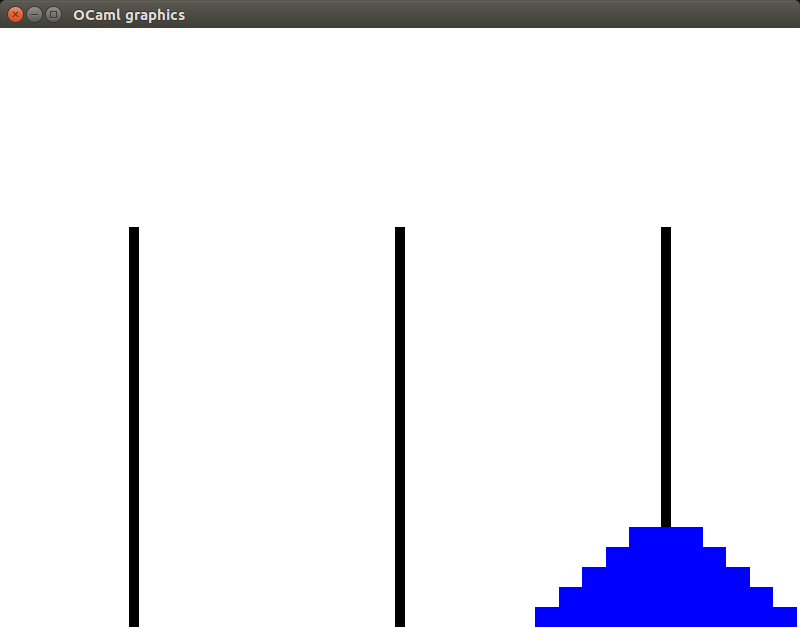
\includegraphics[width=\linewidth]{hanoi_end.png}
			  \caption{État final}\label{fig:hanoi_end}
			\endminipage\hfill
		\end{figure}

		Nous avons choisi pour représenter la situation un tableau de piles
		\texttt{rods}: chaque pile du tableau représente chacun des poteaux et
		contient les disques qui y sont empilés.

		La seule complication du code est le choix du poteau temporaire utilisé
		pour chaque déplacement de disques. La première implémentation réalisée
		repose sur la fonction suivante \texttt{choose}:

		\begin{lstlisting}
		let choose a b =
		  if a = b then failwith "a and b are equal"
		  else if a = 0 then
			if b = 1 then 2
			else 1
		  else if a = 1 then
			if b = 0 then 2
			else 0
		  else if a = 2 then
			if b = 0 then 1
			else 0
		  else failwith "a or b are not between 0 and 2"
		;;
		\end{lstlisting}

		Cette fonction prend en argument deux éléments distincts de {0, 1, 2} et
		renvoie le troisième et est utilisée pour choisir automatiquement dans
		la fonction \texttt{move} le poteau temporaire à utiliser:

		\begin{lstlisting}
		let rec move rods num_discs orig_rod dest_rod =
		  if num_discs = 1 then
			  move_disc rods orig_rod dest_rod
		  else
			(
			  let temp_rod = choose orig_rod dest_rod in
			  move rods (num_discs - 1) orig_rod temp_rod;
			  
			  move_disc rods orig_rod dest_rod;
			  
			  move rods (num_discs - 1) temp_rod dest_rod;
			)
		;;
		\end{lstlisting}

		Lors de l'implémentation de la fonction résolvant le problème des tours
		de Hanoi à n poteaux, nous nous sommes rendu compte que la fonction
		\texttt{choose} était difficilement généralisable. Nous avons donc choisi
		de passer le poteau intermédiaire en argument à la fonction \texttt{move}:

		\begin{lstlisting}
		let rec move rods num_discs orig_rod dest_rod temp_rod=
		  if num_discs = 1 then
			  move_disc rods orig_rod dest_rod
		  else
			(
			  move rods (num_discs - 1) orig_rod temp_rod dest_rod;
			  
			  move_disc rods orig_rod dest_rod;
			  
			  move rods (num_discs - 1) temp_rod dest_rod orig_rod;
			)
		;;
		\end{lstlisting}

		Cette modification permet de choisir comme l'on veut le poteau intermédiaire,
		ce qui est nécessaire pour la version généralisée de l'algorithme.
	
	\subsection{Principe: algorithme généralisé}
		Pour ce problème, l'implémentation choisie est la deuxième présentée.
		
		Cette fois il s'agit d'utiliser au mieux les poteaux supplémentaires.
		Nous avons calculé le nombre de disques pouvant être sur les poteaux
		intermédiaires, pour répartir ces disques sur chacun des poteaux intermédiaires
		en utilisant comme poteau temporaire le dernier (étape 1), ensuite il faut
		déplacer le disque le plus grand sur le dernier poteau (étape 2), et finalement
		il suffit de réaliser le parcours inverse de celui effectué dans l'étape 1,
		et de regrouper les disques intermédiaires sur le dernier poteau (étape 3).
		
		\begin{figure}[!h]
			\minipage{0.24\textwidth}
			  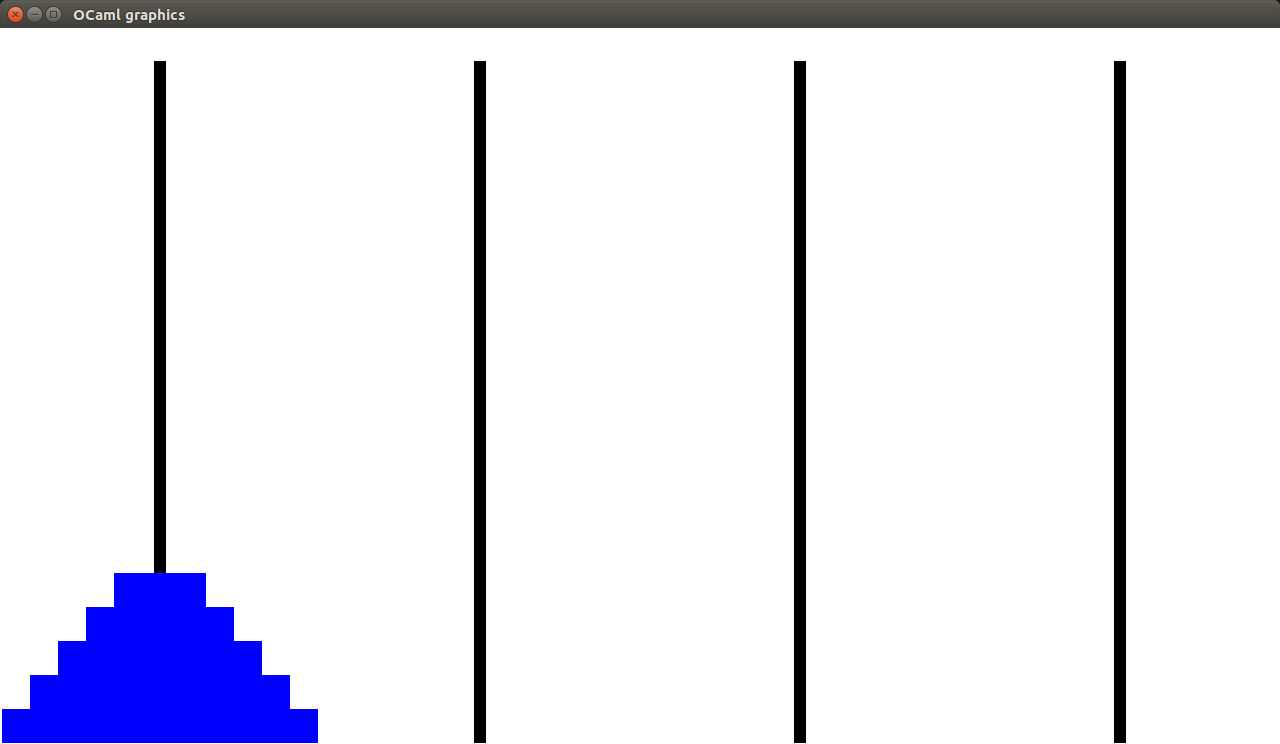
\includegraphics[width=\linewidth]{hanoi_gen_start.png}
			  \caption{État initial}\label{fig:hanoi_gen_start}
			\endminipage\hfill
			\minipage{0.24\textwidth}
			  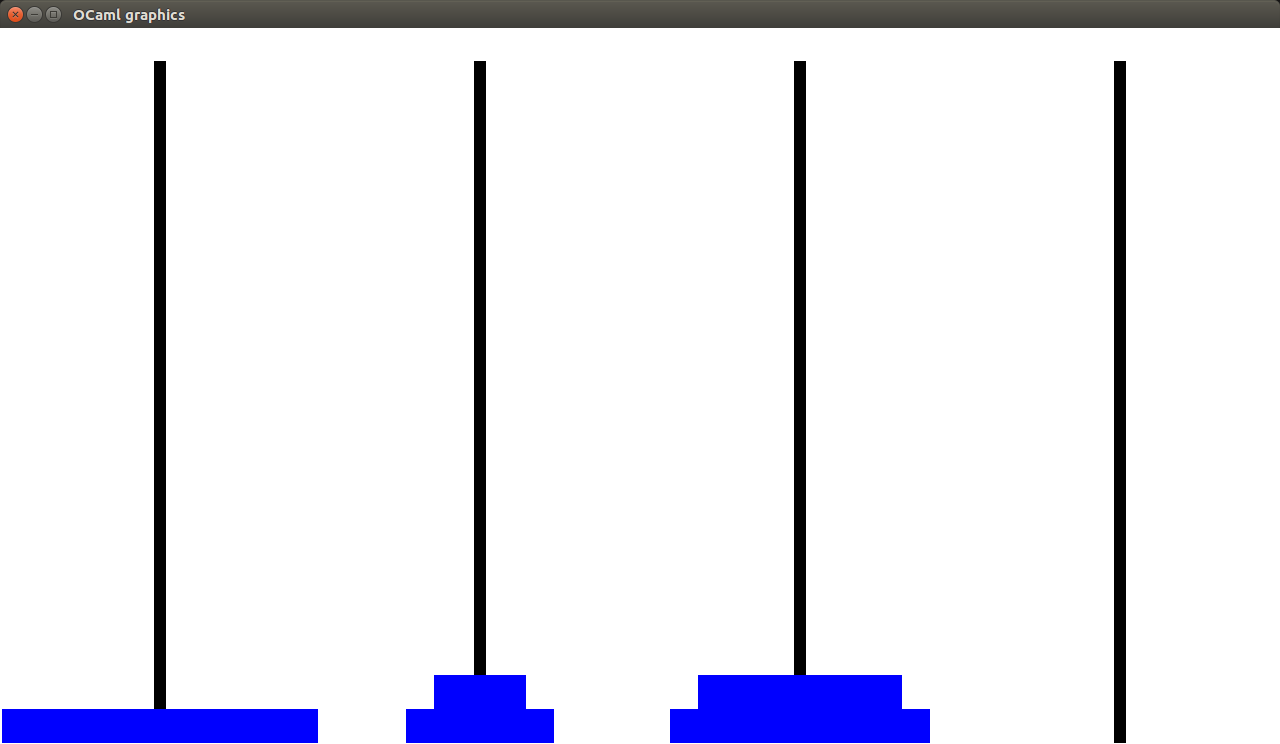
\includegraphics[width=\linewidth]{hanoi_gen_mid1.png}
			  \caption{Fin étape 1}\label{fig:hanoi_gen_mid1}
			\endminipage\hfill
			\minipage{0.24\textwidth}
			  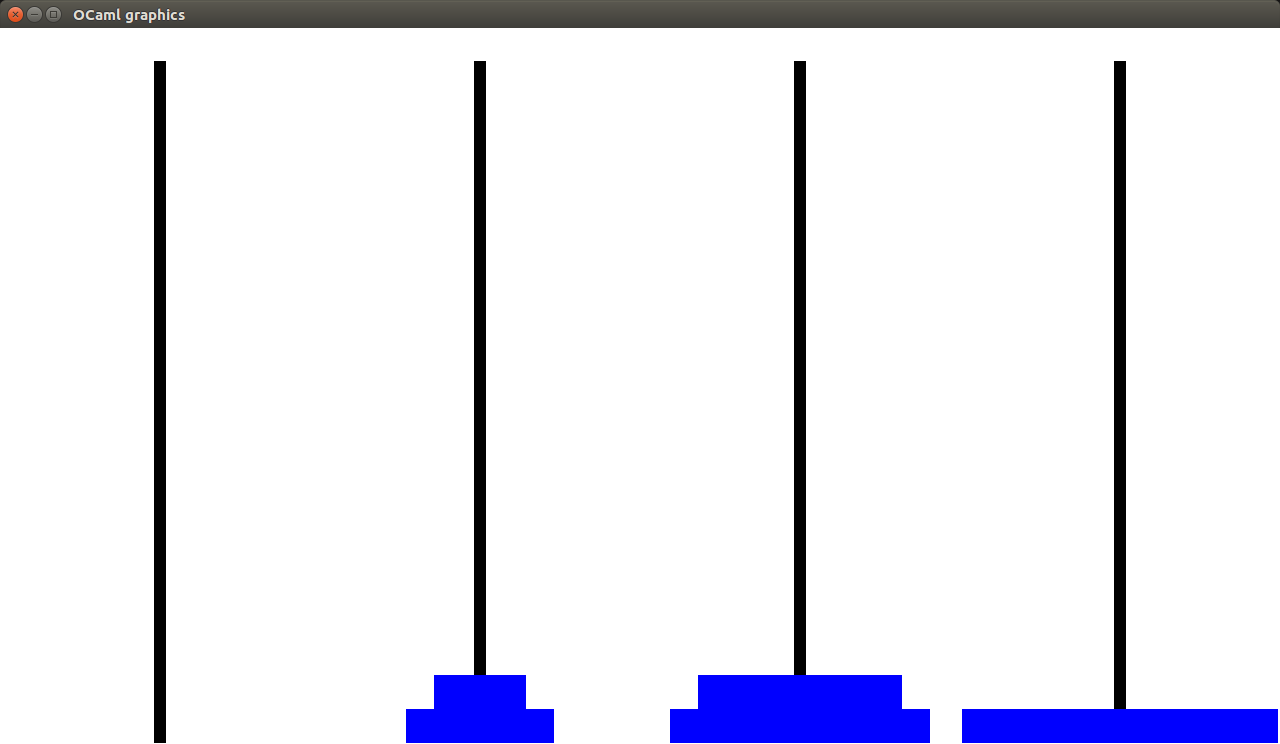
\includegraphics[width=\linewidth]{hanoi_gen_mid2.png}
			  \caption{Fin étape 2}\label{fig:hanoi_gen_mid2}
			\endminipage\hfill
			\minipage{0.24\textwidth}
			  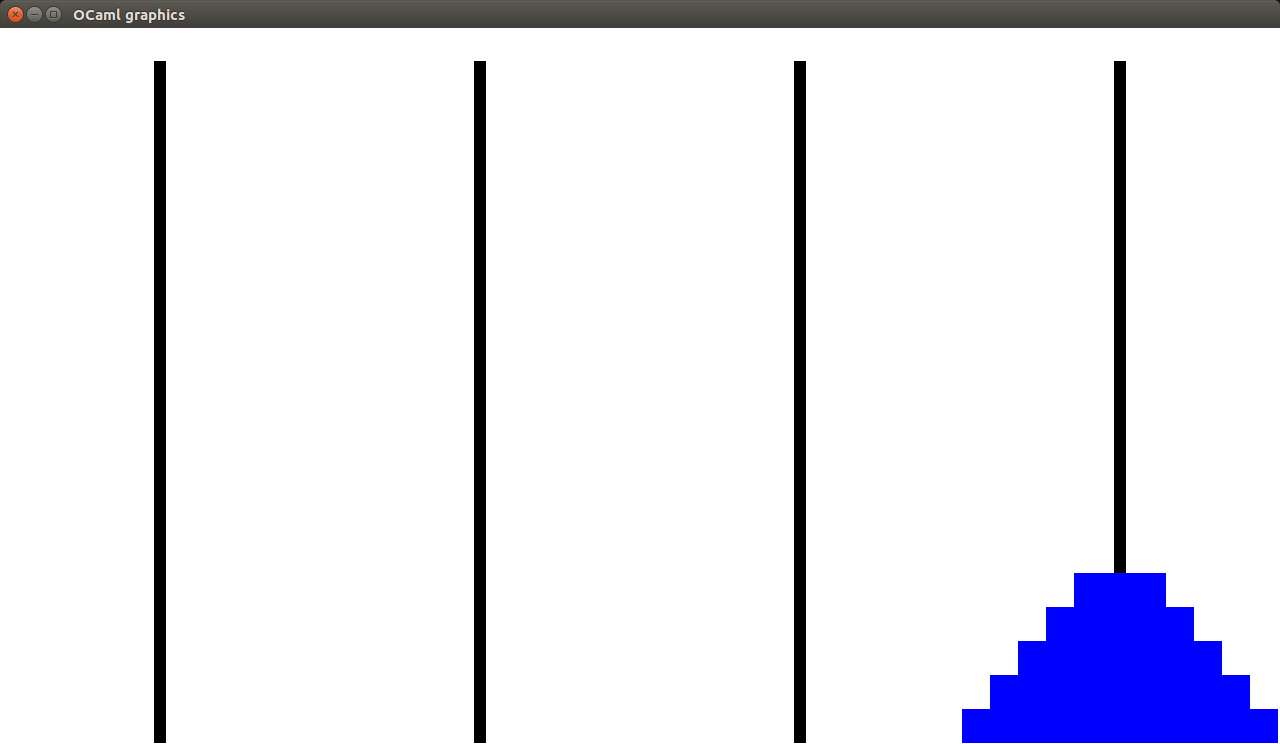
\includegraphics[width=\linewidth]{hanoi_gen_end.png}
			  \caption{État final}\label{fig:hanoi_gen_end}
			\endminipage\hfill
		\end{figure}
		
		Ainsi beaucoup moins de déplacements sont nécessaires pour la résolution
		du problème.

\end{document}

%%%%%%%%%%%%%%%%%%%%%%%%%%%%%%%%%%%%%%%%%%%%%%%%%%%%%%%%%%%%%%%%%%%%%%%%
